
\documentclass{article}
\usepackage{polski} %moze wymagac dokonfigurowania latexa, ale jest lepszy niż standardowy babel'owy [polish]
\usepackage[utf8]{inputenc}
\usepackage[OT4]{fontenc}
\usepackage{graphicx,color} %include pdf's (and png's for raster graphics... avoid raster graphics!)
\usepackage{url}
\usepackage[pdftex,hyperfootnotes=false,pdfborder={0 0 0}]{hyperref} %za wszystkimi pakietami; pdfborder nie wszedzie tak samo zaimplementowane bo specyfikacja nieprecyzyjna; pod miktex'em po prostu nie widac wtedy ramek


% Zmiana rozmiarów strony tekstu
\addtolength{\voffset}{-1cm}
\addtolength{\hoffset}{-1cm}
\addtolength{\textwidth}{2cm}
\addtolength{\textheight}{2cm}

%bardziej zyciowe parametry sterujace rozmieszczeniem rysunkow
\renewcommand{\topfraction}{.85}
\renewcommand{\bottomfraction}{.7}
\renewcommand{\textfraction}{.15}
\renewcommand{\floatpagefraction}{.66}
\renewcommand{\dbltopfraction}{.66}
\renewcommand{\dblfloatpagefraction}{.66}
\setcounter{topnumber}{9}
\setcounter{bottomnumber}{9}
\setcounter{totalnumber}{20}
\setcounter{dbltopnumber}{9}

% własny bullet list z malymi odstepami
\newenvironment{tightlist}{
\begin{itemize}
  \setlength{\itemsep}{1pt}
  \setlength{\parskip}{0pt}
  \setlength{\parsep}{0pt}}
{\end{itemize}}

%obrazkow szukamy w nastepujacym katalogu:
\graphicspath{{pics/}}



% \title{Sprawozdanie z laboratorium:\\Metaheurystyki i Obliczenia Inspirowane Biologicznie}
% \author{}
% \date{}


\begin{document}

\thispagestyle{empty} %bez numeru strony

\begin{center}
{\large{Sprawozdanie z laboratorium:\\
Komunikacja człowiek-komputer\\
}}

\vspace{3ex}

Część I: Python i wizualizacja

\vspace{3ex}
{\footnotesize\today}

\end{center}


\vspace{10ex}

Prowadzący: dr hab.~inż. Maciej Komosiński

\vspace{5ex}

Autor:
\begin{tabular}{lllr}
\textbf{Michał Lewiński} & inf122505 & WI & michal.lewinski@student.put.poznan.pl \\
\end{tabular}

\vspace{5ex}

Zajęcia środowe, 16:50.

\vspace{35ex}

\noindent Oświadczam/y, że niniejsze sprawozdanie zostało przygotowane wyłącznie przez powyższych autora/ów,
a wszystkie elementy pochodzące z innych źródeł zostały odpowiednio zaznaczone i~są cytowane w bibliografii.

\newpage


\begin{figure}
\begin{center}
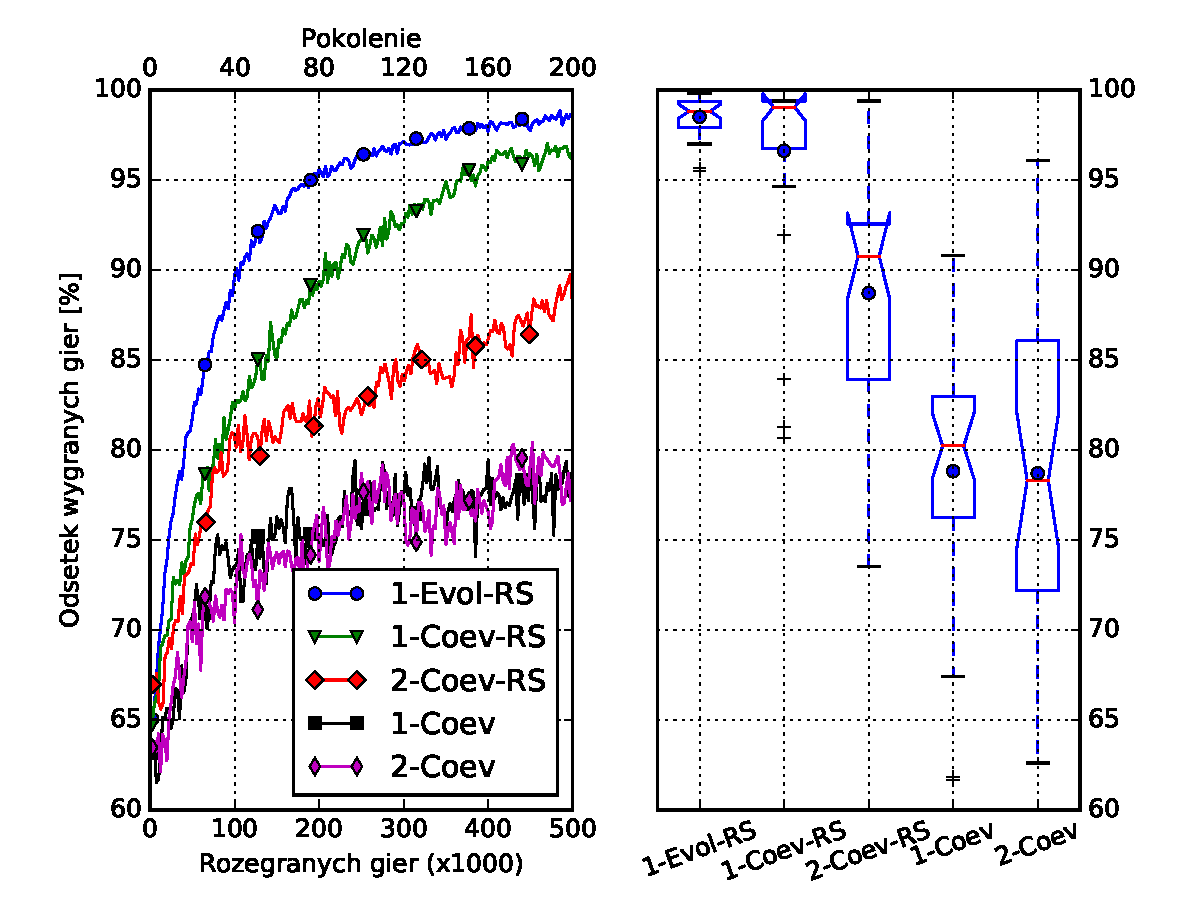
\includegraphics[width=1.0\textwidth]{wykresy.pdf}
\end{center}
\caption{Wykres liniowy przedstawia przebiegi w funkcji ,,czasu", natomiast wykres pudełkowy przedstawia końcowe wyniki algorytmów}
\label{fig:schemat}
\end{figure}


\section{Wstęp}

Pierwsze zadanie laboratoryjne polegało na napisaniu programu w Pythonie, który za pomocą wykresów przedstawi wyniki działania pięciu różnych algorytmów ewolucyjnych. Dane należało wczytać z plików csv, a następnie za pomocą biblioteki \textit{matplotlib} utworzyć wykres liniowy i pudełkowy. W kodzie programu zawarte zostały komentarze, które opisują działanie wykorzystanych funkcji.

\section{Pierwsze programowanie z Pythonem}

Pierwszy projekt w Pythonie był interesującym doświadczeniem. Początkowo miałem problemy z rozróżnieniem wersji Pythona (pip/pip3 oraz python/python3), lecz po udanej instalacji nie napotkałem już żadnych większych problemów. Wykorzystywanie tabulatorów zamiast nawiasów sprawiało mi lekkie trudności ale poprawiły końcową czytelność kodu. Przy tworzeniu programu korzystałem głównie z dokumentacji biblioteki \textit{matplotlib} oraz sekcji podpowiedzi w treści zadania. 

\end{document}
